\documentclass[a4paper,12pt]{article}
\usepackage[MeX]{polski}
\usepackage[utf8]{inputenc}
\usepackage{graphicx}
\usepackage{sidecap}
\usepackage{wrapfig}
\usepackage{times}
\usepackage{textcomp}

%opening
\title{Piłkarzyk}
\author{\texttildelow Adam Rembiewski}

\begin{document}

\maketitle
\section{Jonathan Blondel}
,,Jonathan Blondel'' (ur. 3 kwietnia 1984 w Ypres) – piłkarz belgijski grający na pozycji lewego pomocnika. Mierzy 172 cm wzrostu, waży 72 kg.
\section{Kariera Klubowa}
Blondel jest wychowankiem klubu US Ploegsteert. W 1993 roku podjął treningi w Excelsiorze Mouscron. W~2001 roku zadebiutował w~jego barwach w~Eerste Klasse. W~sezonie 2001/2002 wystąpił w 18 spotkaniach ligowych. 17 sierpnia 2002 Belg podpisał kontrakt z Tottenhamem Hotspur, do którego przeszedł na zasadzie wolnego transferu. W Premiership swój pierwszy mecz zaliczył 31 sierpnia, a Tottenham pokonał Southampton F.C. 2:1. W~Tottenhamie nie miał jednak szans na grę na skutek konkurencji w składzie i~występował głównie w lidze rezerw. Łącznie przez półtora roku pobytu na White Hart Lane zaliczył tylko dwa występy w ekstraklasie Anglii.
\begin{wrapfigure}{r}{0.5\textwidth}
\begin{center}
\vspace{-20pt}
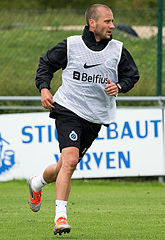
\includegraphics[width=0.1\textwidth,natwidth=165,natheight=240]{fotki/fotka.jpg}
\end{center}
\vspace{-20pt}
\caption{Jonathan Blondel}
\vspace{-10pt}
\end{wrapfigure}
W styczniu 2004 Blondel wrócił do Belgii i~przeszedł do Club Brugge. Kosztował 1,2 miliona euro. Przez pierwsze 2,5 roku w zespole z Brugii był na ogół rezerwowym. W 2004 roku zdobył Puchar Belgii, a w 2005 roku wywalczył swój pierwszy w karierze tytuł mistrza kraju. W~obu przypadkach zdobywał także Superpuchar Belgii. W sezonie 2006/2007 występował w wyjściowej jedenastce Brugge~i~po raz drugi w karierze zdobył puchar kraju. W~2015 zakończył karierę.
\begin{table}
\begin{tabular}{lcllll}
\hline
\textbf{Sezon}&\textbf{Klub}&\textbf{Kraj}&\textbf{Rozgrywki}&\textbf{Mecze}&\textbf{Bramki}\\
\hline
$2001/02$ & Excelsior Mouscron&Belgia&Eerste Klasse&18&0 \\
$2002/03$ & Tottenham Hotspur&Anglia&Premiership&1&0 \\
$2003/04$ & Tottenham Hotspur&Anglia&Premiership&1&0 \\
$2003/04$ & Club Brugge&Belgia&Eerste Klasse&8&0 \\
\hline
\end{tabular}
\caption{Tabela wyników}
\end{table}
\begin{figure}
\centering
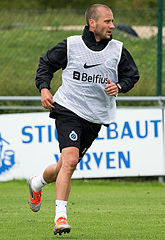
\includegraphics[width=0.1\textwidth,natwidth=165,natheight=240]{fotki/fotka.jpg}
\caption{Jonathan Blondel}
\label{fig:Jonathan Blondel}
Piłkarz \ref{fig:Jonathan Blondel} jest przedstawiony na fotografii.
\end{figure}

\end{document}